\chapter{Cómo opera Spark}

En este apartado vamos a tratar qué sucede internamente cuando estamos trabajando con Spark. Para iniciarnos en dicha materia debemos familiarizarnos antes con algunos conceptos propios de Spark.

\section{Tareas}
Las tareas son unidades de trabajo individuales , cada una enviada a una máquina, es decir, una tarea no se puede ejecutar en más de un executor, cada tarea atacará a una partición específica de los datos. Dicho de otra manera, una tarea es simplemente una unidad de cálculo aplicada a una unidad de datos (partición). Particionar los RDD en un mayor número de particiones significa que se pueden ejecutar más en paralelo, siempre y cuando el clúster tenga recursos suficientes. Spark no puede ejecutar más tareas a la vez que el número de núcleos por executor por la cantidad de executors.El número de tareas por etapa corresponde al número de particiones en el RDD de salida de esa etapa.\\

Cada tarea realiza internamente los mismos pasos:\\

\begin{enumerate}

\item Obtener su entrada, ya sea desde el almacenamiento de datos (si el RDD es un RDD de entrada), un RDD existente (para datos ya almacenados en caché), o salidas de shuffle.\\

\item Realizar la operación necesaria para calcular los RDDs que representa.\\

\item Escribirá la salida de shuffle, en almacenamiento externo o de vuelta al driver (si es el RDD final de una acción como \textit{count()}).
\end{enumerate}

El conjunto de tareas producidas por una transformación con dependencias \textit{narrow} se denomina etapa.\\

\section{Etapas}
Para ser más eficiente, Spark agrupa las operaciones que pueden ser aplicadas en una sola partición, y, consecuentemente, en una única máquina sin que sea necesaria comunicación en red entre los nodos esclavos, esto es, cuando no se requiere información de otras máquinas. Es decir, canaliza juntas las transformaciones con dependencias \textit{narrow}, mientras que las transformaciones con dependencias \textit{wide} suponen el límite entre una etapa y otra.\\

En consecuencia, entre una etapa y el siguiente se necesita comunicación con el driver, por lo que se han de ejecutar en secuencia. Sin embargo, en casos donde no se requiera información de otra etapa, por ejemplo, aplicar operaciones a dos RDD sin ningún padre común, se pueden calcular en paralelo.\\

\begin{figure}[H]
	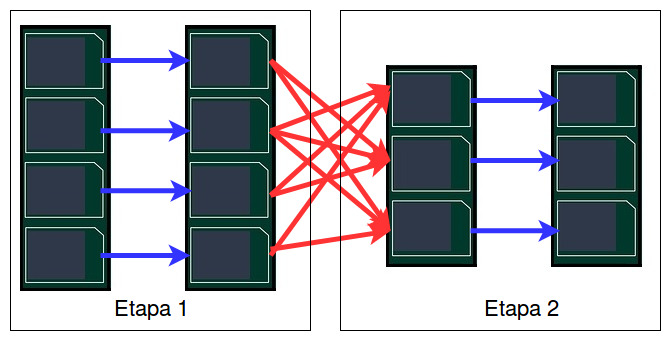
\includegraphics[scale=0.6]{img/etapas} 
	\centering
	\caption{Límite entre dos etapas}
	\label{etapas}
\end{figure}

Podemos clasificar las etapas en dos categorías diferentes, según lo que marque su final:\\

\begin{itemize}
\item ShuffleMapStage, que escribe los archivos de salida de shuffle.
\item ResultStage, para la etapa final que ejecuta una acción.
\end{itemize}

Las agrupaciones de etapas fruto de una acción se conocen como trabajo. Las etapas suelen compartirse en varios trabajos, si estos trabajos reutilizan los mismos RDD.\\

\section{Trabajo}
Suponen el elemento más alto de la jerarquía de ejecución de Spark. Cada trabajo de Spark corresponde a una acción, y suponen el desencadenante para comenzar el cómputo sobre los RDD, debido al carácter perezoso de estos. \\

\section{Aplicación}
Por último, definimos a cada uno de los programas en los que se crea un SparkContext como una aplicación de Spark. Entre diferentes aplicaciones no se comparte memoria ni recursos.\\

Ahora que ya conocemos las distintas fases por las que pasa toda aplicación de Spark, falta por abordar una cuestión. Como hemos visto, la memoria entre etapas no puede ser compartida por no estar en la misma máquina virtual, por lo que nos surge la pregunta de cómo compartir información entre etapas. La respuesta sería escribiendo a disco, operación conocida como shuffle.\\

\section{Shuffle}
Según la documentación oficial de Spark, el shuffle es “el mecanismo de Spark para redistribuir los datos de manera que se agrupen de manera diferente en las particiones”. Es conveniente aclarar que no todo movimiento de datos por el clúster es considerado como shuffle. Las acciones, escrituras o lecturas de una fuente externa no se consideran shuffle. La fase de shuffle representa una repartición física de los datos, esto es, conlleva escritura en disco. Esto contradice la definición inicial que dimos de Spark como  motor de computación en memoria, pero se trata de momentos concretos en los que debido a una transformación con dependencias \textit{wide}, es decir, cuando necesite combinar los datos de distintas etapas, o por saturación de memoria, en vez de mantener los datos cacheados los escribe temporalmente a disco, tras lo cual se genera una nueva etapa con un nuevo conjunto de particiones.\\

Su comportamiento varía dependiendo del Shuffle Manager que usemos y cada uno tendrá su Caso de Uso. Tratar los diferentes shuffle manager va más allá de lo que pretendemos abordar en este texto, por lo que únicamente nos centraremos en las propiedades generales.\\

Operaciones que pueden causar shuffle son aquellas que implican una repartición de los datos entre particiones, como repartition y coalesce, operaciones \textit{ByKey}, excepto  \textit{countByKey} y operaciones de mezcla de RDDs como \textit{cogroup} y \textit{join}.\\

Se trata de una operación muy costosa, pues debe leer todas las particiones para encontrar todos los valores de todas las claves, y luego unir los valores de las particiones para calcular el resultado final de cada valor, esto conlleva escritura y lectura en disco, serialización de datos y movimiento de entrada y salida por la red \cite{6RDD_Documentation}.\\

La fase de shuffle se desarrolla en dos partes: map y reduce. En la parte de map, Spark genera archivos intermedios que son escritos en disco en la ruta local de cada nodo. Estos archivos son conservados hasta que los RDD a los que corresponden ya no se utilizan, de esta manera, en caso de fallo no es necesario que vuelvan a ser calculados. Cada tarea map escribe un archivo por cada tarea Reduce. El directorio de almacenamiento temporal en disco puede ser configurado en la propiedad spark.local.dir que se configura a nivel de application. Además, spark brinda la opción de comprimir los archivos de salida Map, especificados por el parámetro \textit{spark.shuffle.compress}.\\

Un efecto de lado, provocado por esta persistencia en disco durante la fase de shuffle, es que la ejecución de un nuevo trabajo sobre los datos que ya se han pasado por la fase shuffle, no vuelve a ejecutar la parte map del shuffle. Debido a que los archivos shuffle ya se habían escrito anteriormente en disco, Spark sabe que puede usarlos para ejecutar únicamente la parte reduce del shuffle. Pese a esta optimización automática,  para un mejor rendimiento es preferible realizar su propio almacenamiento en caché con el método caché, que le permite controlar exactamente qué datos guardar y dónde.\\

Durante la fase de reduce, Spark requiere que todos los datos quepan en memoria. Cuando la memoria requerida de cada tarea reduce excede la asignada, se emite una excepción de falta de memoria y se debe interrumpir todo el trabajo. Para evitar quedarse sin memoria, se debe especificar un valor suficientemente alto para la cantidad de tareas reduce.\\

Llegados a este punto ya estamos en disposición de poder analizar qué sucede internamente durante una aplicación de Spark:\\

El código escrito por un usuario define un DAG de RDD. En primer lugar, Spark comprueba si el código escrito por el usuario es válido. Tras esto, Spark lo convierte en un flujo lógico de operaciones, el plan lógico \cite{6DAGandPE} (también conocido como DAG de dependencias). Cuando se realiza una acción este plan lógico se pasa a través de SparkContext al DAG Scheduler, que lo usa para crear un plan de ejecución físico, el DAG de etapas, que consiste en tareas agrupadas en etapas, las cuales son enviadas como TaskSets a una implementación TasScheduler subyacente, que es el encargado de enviar las tareas para su ejecución en el clúster a través del cluster manager \cite{6DFariDAG}. En este punto Spark ejecuta este plan en el clúster.\\

Spark cuenta con mecanismos internos para optimizar tanto el plan lógico como el plan físico, y también realiza optimizaciones en tiempo de ejecución. Estos difieren en función de si estamos tratando con las APIs estructuradas o con RDDs. En cualquier caso, el plan físico siempre es ejecutado sobre RDDs.
